
% This LaTeX was auto-generated from MATLAB code.
% To make changes, update the MATLAB code and republish this document.

\documentclass{article}
\usepackage{graphicx}
\usepackage{color}

\sloppy
\definecolor{lightgray}{gray}{0.5}
\setlength{\parindent}{0pt}

\begin{document}

    
    
\subsection*{Contents}

\begin{itemize}
\setlength{\itemsep}{-1ex}
   \item �rednia
\end{itemize}
\begin{verbatim}
 clear all; % comparison2mean.m

[Yemp, data, time, x, lTim, lrT] = dane();

OrgYemp = Yemp;
Ldanych = length(x); % size(x, 2);
T = max(x) - min(x) + 1; sred_temp = mean(Yemp);
Yemp = dtrend(Yemp, 1); %sredAfterDentrend = mean(Yemp);
sigYf = std(Yemp);

% G��bokie my�lenie = prezentacja danych + wyobra�enia
kol1 = 'r*'; if(Ldanych > 80) kol1 = 'r.'; end
figure(2), subplot(2, 1, 1);
plot(x, Yemp + sred_temp, kol1); ylabel('[*C]'); title('Regresja harmonicznych'); hold on

% z = input(' ? jaka to funkcja ? !!!  <Ent> - co mogloby byc ?');

% za�. funkcji harmonicznej
nrOm = [7 14 21 28 56]; %nrOm;%[1 2 5 20 36 42 134 236 500 600];

om = 2 * pi / T * nrOm;
% %% Projekt modelu - oblicz FId
[FId, Ldanych, Lh, Kd] = modelRharm(x, om); % za�. funkcji harmonicznej
% doda� dane z dziurami
% =============== wybieramy model: Lhm i Km ===================
Lhm = 5;
% =============================================================
Yemp = Yemp';
Km = 2 * Lhm; % Przyjety (arbitralnie) rzad modelu  Kolumny Macierzy
FI(:, 1:Km) = FId(:, 1:Km);
% dalej ju� tylko numeryka i grafika
Gd = FI' * FI;
G = inv(Gd);

Ao = G * FI' * Yemp; % Wsp.A=inv(FItransp*FI)*FItransp*Yempiryczne
% sprawdz modelu
Yo = FI * Ao;
Em = Yemp - Yo;

if (1) E = Em; LdE = Ldanych;
else E(x') = Em; LdE = length(E); % uzupe�niamy braki zerami;
end

varE = (E' * E) / (LdE - Km);
sigEo = sqrt(varE);

% ============= model AR reszt ======================
alf = E(2:end)' * E(1:end - 1) / ((LdE - 1) .* varE);
Talf = -1 / log(alf); txalf = '\alpha';
v(LdE, 1) = 0;
v(1, 1) = 0; for(n = 2:LdE) v(n, 1) = E(n - 1) * alf; end;
sigZ = std(E - v);
% ........................................................
% obliczanie sigYo i sigYe;
KA = G * varE; % macierz kowariancji wspolcz.
Lduzych = 0;

for (n = 1:Ldanych)
    varYo = FI(n, :) * KA * FI(n, :)';
    sigYo(n, 1) = sqrt(varYo);
    sigYe(n, 1) = sqrt(varYo + varE);
    if (abs(E(n)) > sigYe(n)) Lduzych = Lduzych + 1; end
end

Kz = sigEo * sqrt(1 - alf^2);

uLd = Lduzych / Ldanych * 100;
% ................................
hold on; if(Ldanych > 30) kol = 'b'; else kol = 'bo-'; end
plot(x, Yemp + sred_temp, 'k.', x, Yo + sred_temp, kol, [x(1) x(end)], [sred_temp sred_temp], 'k:'); %axis('tight');
plot(x, Yo + sred_temp + sigYo, 'b--', x, Yo + sred_temp - sigYo, 'b--');
plot(x, Yo + sred_temp + sigYe, 'm--', x, Yo + sred_temp - sigYe, 'm--');
hold off; axis('tight')
xlabel(sprintf('Ldanych = %d [7 lat]', Ldanych));
\end{verbatim}

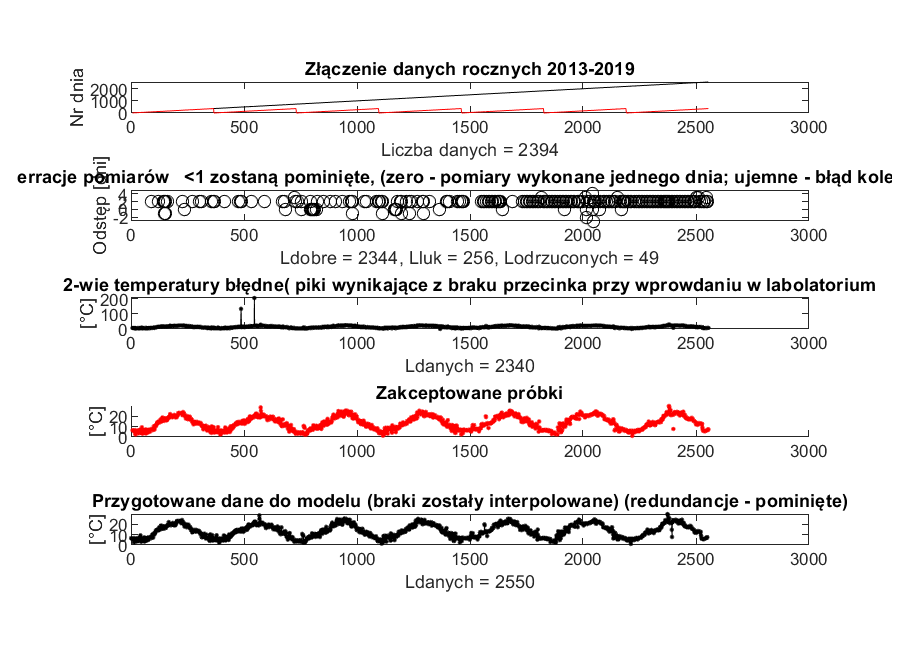
\includegraphics [width=4in]{comparison2mean_01.eps}

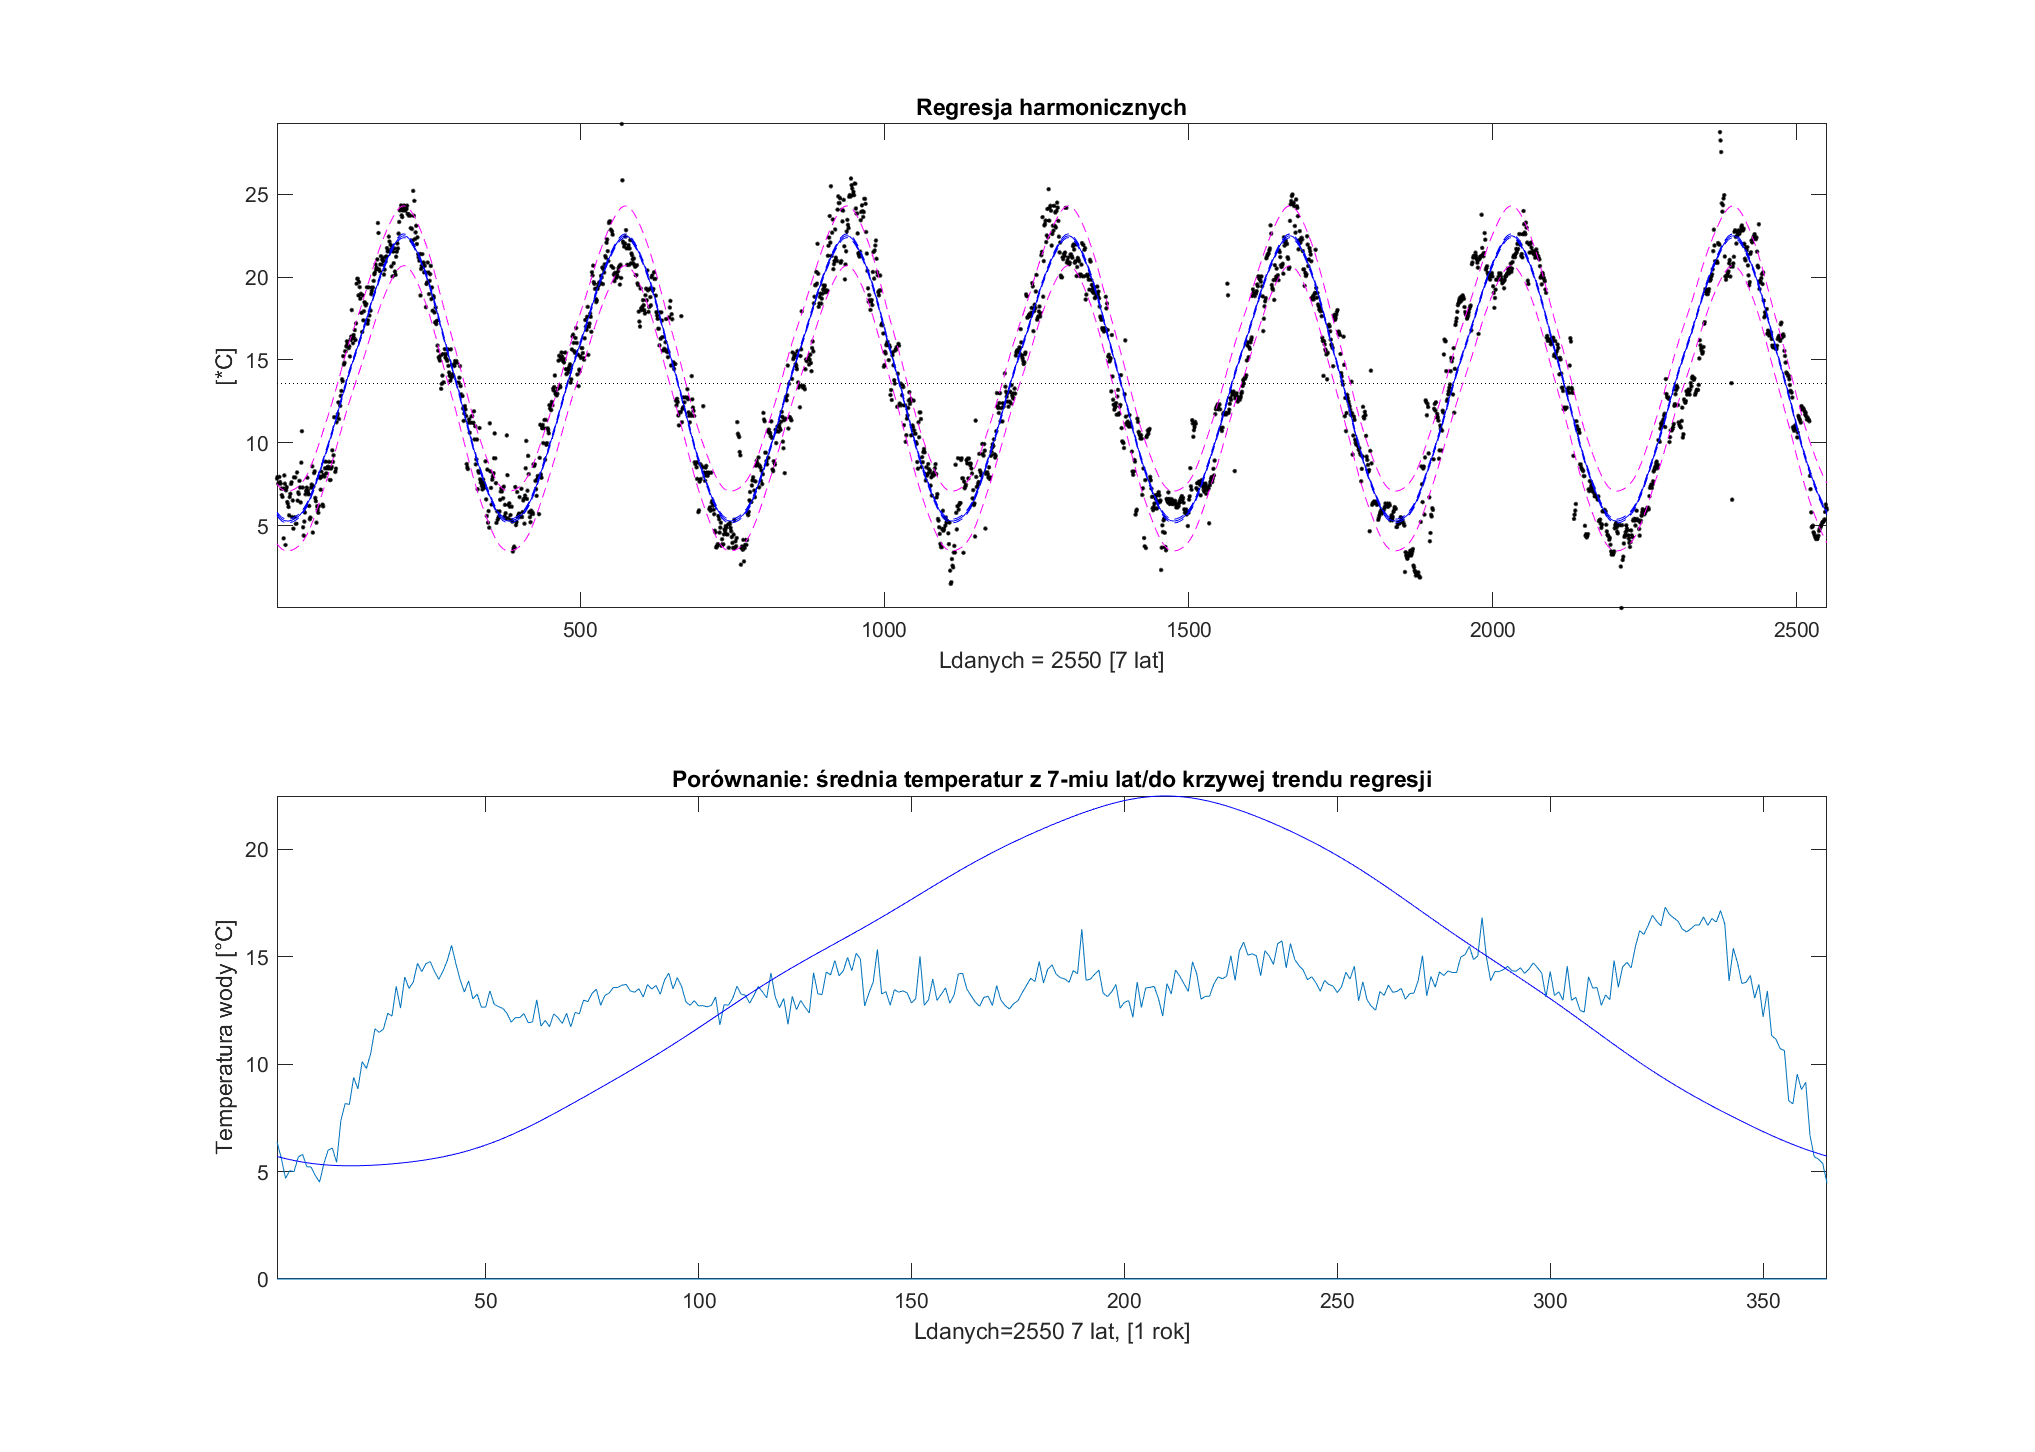
\includegraphics [width=4in]{comparison2mean_02.eps}


\subsection*{�rednia}

\begin{verbatim}
figure(2), subplot(2, 1, 2),
sr = zeros(365);
for(i=1:7)
    for(k=1:365)
        if (i*k > 2550) break; end;
        sr(k)=sr(k)+OrgYemp(i*k);
    end
end

plot(sr/7); hold on;
plot( [1:365], Yo(1:365) + sred_temp, kol);

xlabel(sprintf('Ldanych=%d, �rednia z 7-miu lat, [1 rok]', Ldanych)); ylabel(['Temperatura wody [' char(176) 'C]']);
axis('tight'); title('Por�wnanie: �rednia temperatur z 7-miu lat/do krzywej trendu regresji'); hold off;
\end{verbatim}

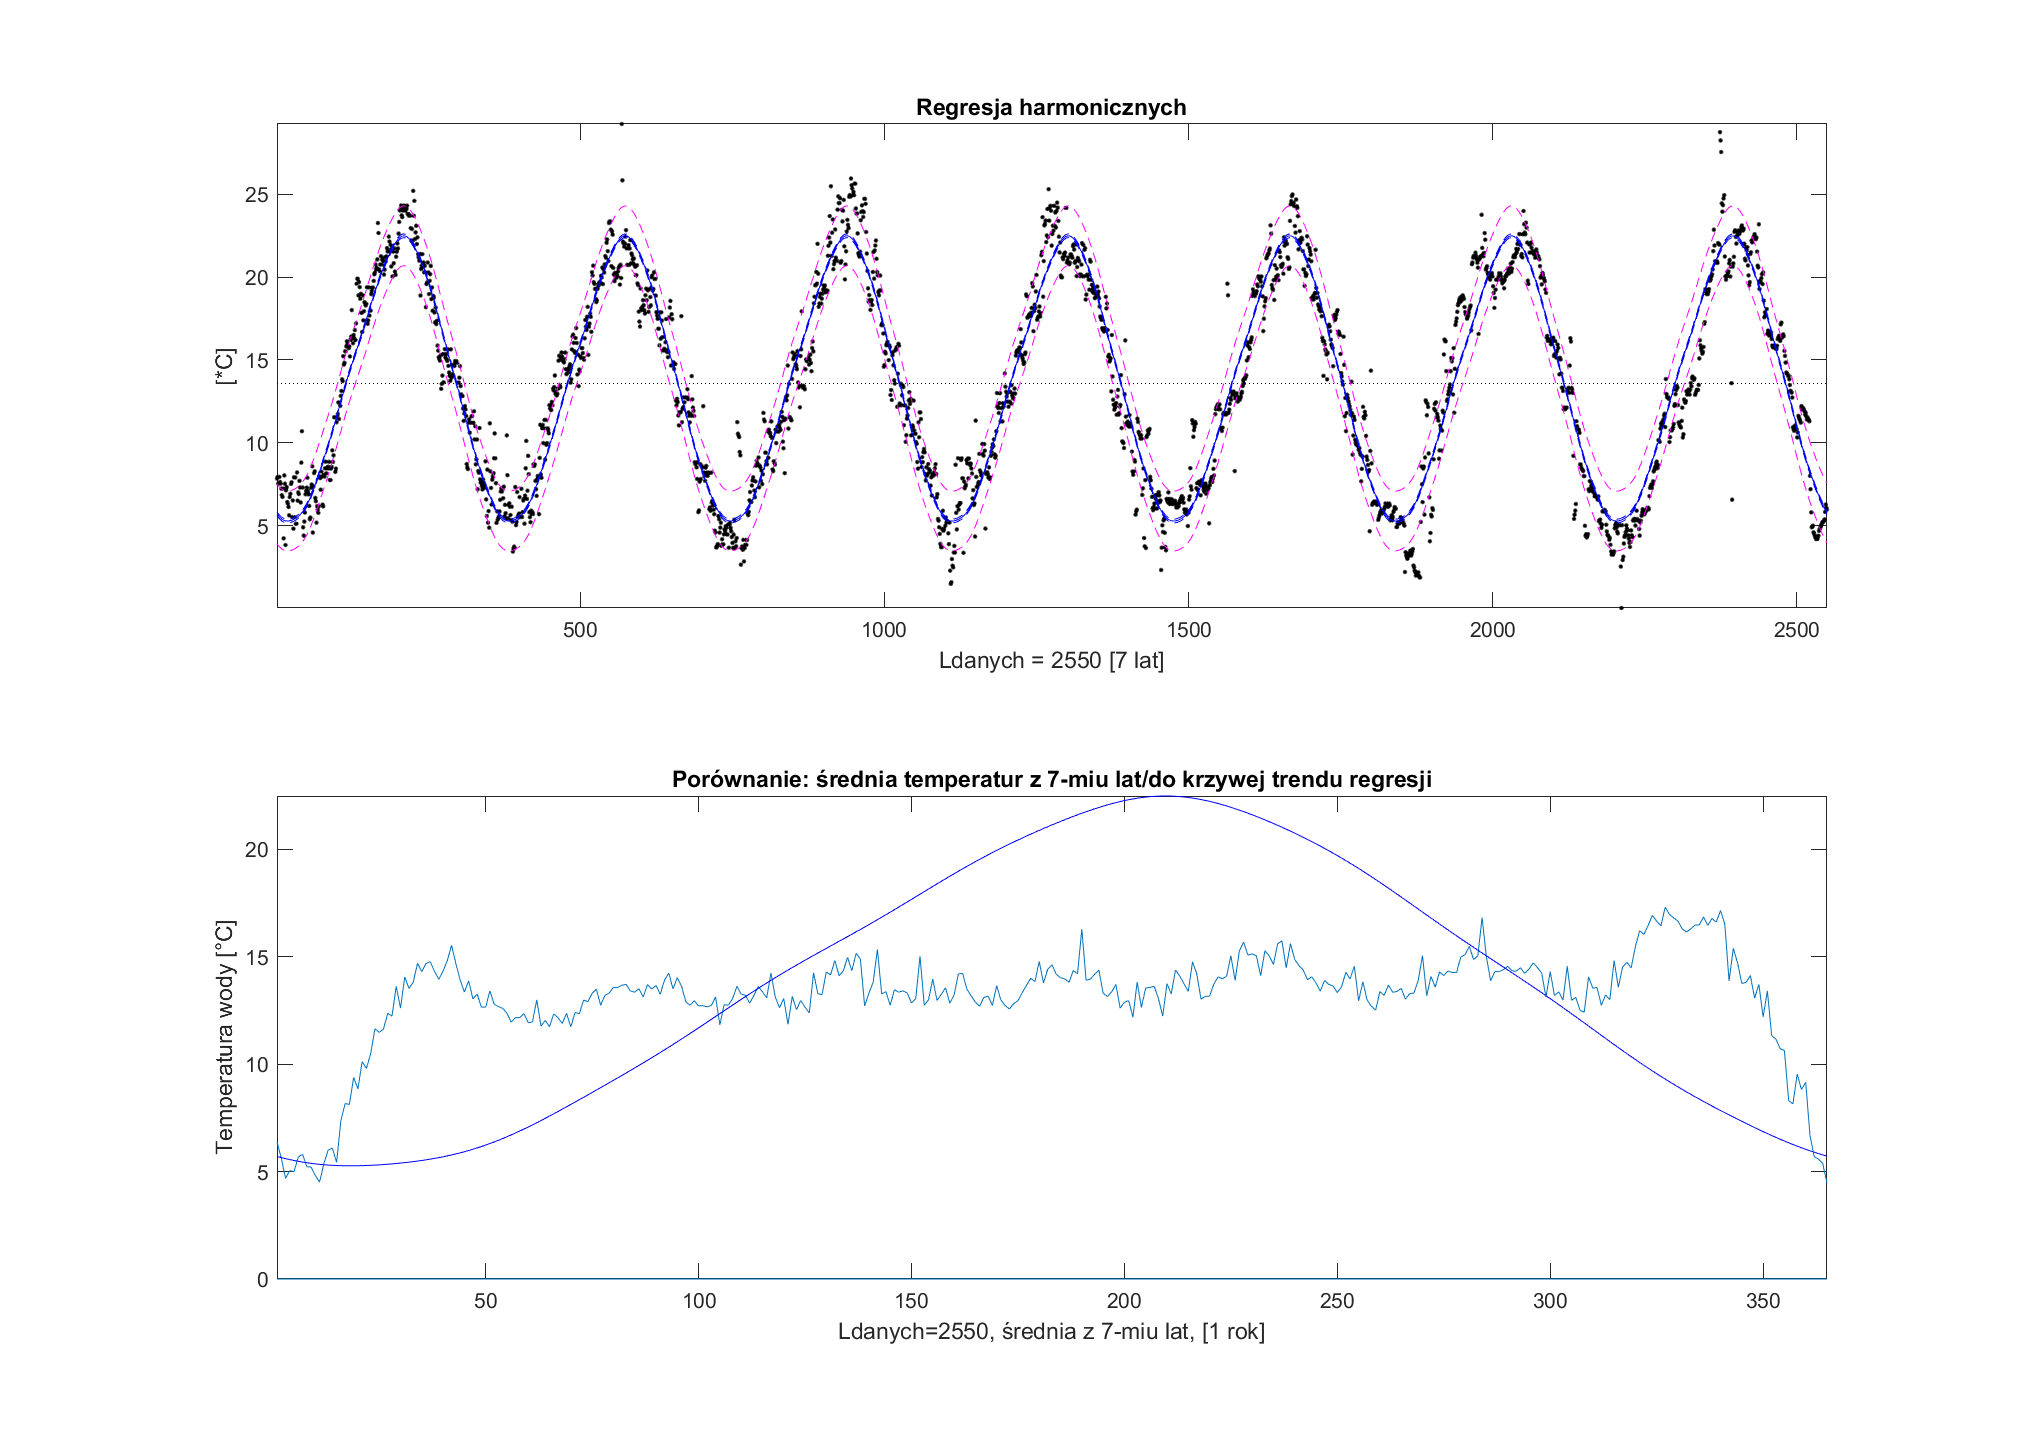
\includegraphics [width=4in]{comparison2mean_03.eps}



\end{document}
    
